\section[Non-Linear Problems]{Non-Linear Problems}

\begin{frame}{Non-Linear Problems}
	In this section, we will explore:
	\begin{itemize}
		\item How to adapt the definition of an artificial neuron to prepare it for the \textbf{gradient backpropagation} learning algorithm.
		\item How to build a \textbf{network} of neurons to solve non-linear problems.
		\item How to adapt the structure of an artificial neuron for \textbf{regression} tasks.
	\end{itemize}
\end{frame}

\subsection[Differentiability]{Differentiability}

\begin{frame}{From the Heaviside Function to the Logistic Function}
	The gradient backpropagation algorithm, which will be covered later in this course, fundamentally relies on computing \textbf{gradients}. The Heaviside step function possesses \textbf{zero} gradients everywhere they exist. This characteristic makes it an incredibly poor choice for neural networks trained via backpropagation. We therefore replace it with a smooth, differentiable \textbf{logistic} function:
	
	\begin{figure}
		\centering
		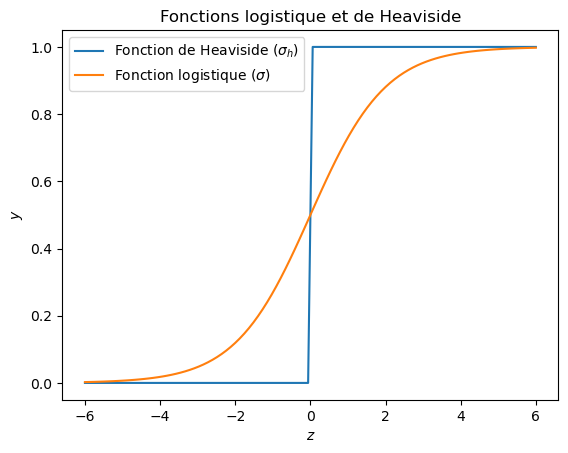
\includegraphics[height=0.4\linewidth]{Images/nonlinearites01}
		\label{fig:nonlinearites01}
	\end{figure}	
\end{frame}

\begin{frame}{New Formulation of an Artificial Neuron}
	Using the logistic function, the mathematical expression of an artificial neuron becomes:
	
	\begin{equation*}
		\hat{y} = \logistic{x \cdot w + b}
	\end{equation*}
	
	\vfill
	\pause
	This is \textbf{exactly} the formulation of logistic regression! The backpropagation method allows us to compute the partial derivatives of the prediction error with respect to the weights $w$ and the bias $b$. Once these gradients are obtained, optimization is carried out using standard \textbf{gradient descent methods}. Such an artificial neuron shares the exact same functional form and learning framework as logistic regression. They are \textbf{rigorously} identical.
\end{frame}

\begin{frame}{Difference from Logistic Regression}
	The divergence from classical logistic regression lies entirely in the strategic approach used to resolve non-linearly separable tasks:
	\begin{itemize}
		\item Logistic regression relies on manual feature expansion or explicit mapping functions on the inputs $X$ to inject non-linearities into the model.
		\item In the neural network paradigm, non-linear mappings are achieved intrinsically by combining layers of simple neurons into an interconnected \textbf{network}.
	\end{itemize}
\end{frame}

\subsection[Network Architecture]{Network Architecture}

\begin{frame}{A Common Abuse of Notation in Neural Networks}
	We commonly write the following expression to denote the vertical stacking of observations through an artificial neuron:
	
	\begin{equation*}
		\hat{Y} = \logistic{X \cdot w + b}
	\end{equation*}
	
	From a strict matrix algebra perspective, this is an abuse of notation. Given that $X \in \mathcal{M}_{n,p}(\R)$, $\hat{Y} \in \mathcal{M}_{n,1}(\R)$, $w \in \mathcal{M}_{p,1}(\R)$, and $b \in \R$, one cannot rigorously add a matrix product to a scalar constant.
	
	\vspace{0.2cm}
	\pause
	
	This convention stems from the computer science world. Computational linear algebra libraries (such as NumPy or PyTorch) utilize a mechanism called \textbf{broadcasting}, which automatically replicates the dimensions of an operand across vectors, matrices, and tensors. Mathematically, the actual operation being executed is:
	
	\begin{equation*}
		\hat{Y} = \logistic{X \cdot w + b \cdot \mathbf{1}_n}
	\end{equation*}
	
	Where $\mathbf{1}_n \in \mathcal{M}_{n,1}(\R)$ represents a column vector of ones: $\mathbf{1}_n = \begin{pmatrix} 1 & 1 & \cdots & 1 \end{pmatrix}^T$.
\end{frame}

\begin{frame}{Assembling Neurons into Layers}
	In this course, we will restrict our focus to \textbf{dense} networks, also widely known as \textbf{fully connected} neural networks.
	
	\vspace{0.3cm}
	
	These architectures organize individual mathematical neurons into distinct, sequential \textbf{layers}.
	
	\vspace{0.3cm}
	
	Such a model is still frequently termed a \textbf{Multilayer Perceptron} (MLP) for historical continuity, even though the structural units have long replaced the Heaviside step function with smooth, continuous logistic or alternative \textbf{activation} functions.
\end{frame}

\begin{frame}{Assembling Neurons into Layers}
	Stacking all observations vertically yields the following compact matrix notation for a single hidden layer within the network:
	
	\begin{block}{A Layer of Neurons in a Dense Architecture}
		Information propagates from layer $k$ ($X^{[k]}$) to layer $k+1$ ($X^{[k+1]}$) during a \textbf{forward pass}. The dimensionality of the data matrix shifts between layers: $X^{[k]} \in \mathcal{M}_{n,p^{[k]}}(\R)$ and $X^{[k+1]} \in \mathcal{M}_{n,p^{[k+1]}}(\R)$. The layer's \textbf{weight matrix} is denoted by $W^{[k+1]} \in \mathcal{M}_{p^{[k]},p^{[k+1]}}(\R)$, and the \textbf{bias vector} is $b^{[k+1]} \in \mathcal{M}_{1,p^{[k+1]}}(\R)$:
		\begin{equation*}
			X^{[k+1]} = \logistic{X^{[k]} W^{[k+1]} + b^{[k+1]}}
		\end{equation*}
		Warning: In this vectorised stacking, the bracketed superscripts $[k]$ and $[k+1]$ identify the explicit layer index within the network topology, not the observations.
	\end{block}
\end{frame}

\begin{frame}{Broadcasting within a Layer of Neurons}
	To visualize the matrix operations clearly, let us unpack the implicit broadcasting hidden inside the layer equation:
	
	\begin{equation*}
		X^{[k+1]} = \logistic{X^{[k]} W^{[k+1]} + b^{[k+1]}}
	\end{equation*}
	
	Here, the matrix product $X^{[k]} W^{[k+1]}$ evaluates to a matrix of dimensions $n \times p^{[k+1]}$, while $b^{[k+1]}$ is a row vector of dimensions $1 \times p^{[k+1]}$. The software execution engine expands the operation as follows:
	
	\begin{equation*}
		X^{[k]} W^{[k+1]} + \left.
		\smash[b]{\underbrace{
				\begin{pmatrix}
					\text{---} & b^{[k+1]} & \text{---} \\
					\text{---} & b^{[k+1]} & \text{---} \\
					\vdots & \vdots & \vdots \\
					\text{---} & b^{[k+1]} & \text{---}
				\end{pmatrix}
			}_{p^{[k+1]} \text{ columns}}}
		\right\} n \text{ rows}
		\vphantom{\underbrace{\begin{matrix} \\ \\ \\ \end{matrix}}_{p^{[k]} \text{ columns}}}
	\end{equation*}
	
\end{frame}

\begin{frame}{Architecture of a Layer of Neurons}
	\begin{center}
		\resizebox{0.85\textwidth}{!}{
			\begin{tikzpicture}[x=1.5cm, y=1.2cm, >=Stealth]
				
				% --- Styles ---
				\tikzset{
					input/.style={circle, draw=black, minimum size=0.8cm, inner sep=0pt, font=\small},
					neuron/.style={circle, draw=black, minimum size=1cm, inner sep=0pt},
					weight/.style={font=\small, text=red!70!black, fill=white, inner sep=1pt, rounded corners}
				}
				
				% --- 1. Inputs ---
				\node[input] (x1) at (0, 3) {$x_1^{(i)[k]}$};
				\node[input] (x2) at (0, 1.5) {$x_2^{(i)[k]}$};
				\node (xdots) at (0, 0) {$\vdots$};
				\node[input] (xp) at (0, -1.5) {$x_{p^{[k]}}^{(i)[k]}$};
				
				\node[anchor=south, font=\scriptsize\bfseries] at (x1.north) {Layer $X^{[k]}$};
				
				% --- 2. Layer Container ---
				\draw[dashed, gray!50, rounded corners=10pt, fill=blue!2] (2.2, -2.7) rectangle (5.5, 4.5);
				\node[font=\scriptsize\bfseries, text=gray!80!black] at (3.85, 4.2) {Dense Layer (3 neurons)};
				
				% --- 3. Neuron Nodes Generation ---
				\foreach \j/\y in {1/3, 2/0.75, 3/-1.5} {
					
					% Linear Summation Node
					\node[neuron, fill=white] (sum\j) at (3, \y) {$\displaystyle \sum$};
					
					% Non-linear Activation Node
					\node[neuron, fill=white] (act\j) at (4.7, \y) {};
					
					% Sigmoid S-curve drawing inside node
					\draw[thick, blue] ([xshift=-0.25cm, yshift=-0.25cm]act\j.center) 
					.. controls ([xshift=0.1cm, yshift=-0.25cm]act\j.center) and ([xshift=-0.1cm, yshift=0.25cm]act\j.center) .. 
					([xshift=0.25cm, yshift=0.25cm]act\j.center);
					
					% Internal state transfer (z)
					\draw[->, thick] (sum\j) -- (act\j) node[midway, above, font=\small] {$z_{\j}^{(i)[k+1]}$};
					
					% Output
					\node (y\j) at (6.5, \y) {$x_{\j}^{(i)[k+1]}$};
					\draw[->, thick] (act\j) -- (y\j);
					
					% Local Bias Input
					\node[input, fill=green!10, draw=green!60!black, minimum size=0.4cm, font=\tiny] (b\j) at (3, \y+0.9) {$+1$};
					\draw[->, green!60!black, thick] (b\j) -- (sum\j) node[midway, right, font=\small] {$b_{\j}^{[k+1]}$};
				}
				
				\node[anchor=south, font=\scriptsize\bfseries] at (y1.north) {Layer $X^{[k+1]}$};
				\node[anchor=north, font=\small, text=blue, align=center] at (act3.south) {Logistic\\$\sigma(z)$};
				
				% --- 4. Synaptic Connections ---
				% Background connections (faded)
				\foreach \y in {1, 2, 3} {
					\draw[->, gray!40] (x1) -- (sum\y);
					\draw[->, gray!40] (x2) -- (sum\y);
					\draw[->, gray!40, dashed] (xdots) -- (sum\y);
					\draw[->, gray!40] (xp) -- (sum\y);
				}
				
				% Highlighted connections for matrix index clarity
				\draw[->, gray!80, thick] (x1) -- (sum1) node[pos=0.25, above, weight] {$w_{1,1}^{[k+1]}$};
				\draw[->, gray!80, thick] (xp) -- (sum3) node[pos=0.25, below, weight] {$w_{3,p^{[k]}}^{[k+1]}$};
				
			\end{tikzpicture}
		}
	\end{center}
\end{frame}

\begin{frame}{Architecture of a Multilayer Perceptron (MLP)}
	To keep complete network schematics clean and readable, we will omit visual bias nodes from this point forward. A node labeled $\Sigma$ now encompasses both the linear weighted summation and its corresponding scalar bias:
	\begin{center}
		\resizebox{1.0\textwidth}{!}{
			\begin{tikzpicture}[x=2cm, y=1.3cm, >=Stealth]
				
				% --- Styles ---
				\tikzset{
					input/.style={circle, draw=black, minimum size=0.8cm, inner sep=0pt, font=\small},
					sum/.style={circle, draw=black, minimum size=0.8cm, inner sep=0pt, fill=white},
					act/.style={circle, draw=blue!80, minimum size=0.8cm, inner sep=0pt, fill=blue!5},
					link/.style={->, red!70!black, opacity=0.4, thick},
					internal/.style={->, gray!60, thick}
				}
				
				% --- 1. Input Layer (3 inputs) ---
				\foreach \i in {1, 2, 3} {
					\node[input] (x\i) at (0, 4-\i*1.2) {$x_\i^{(i)}$};
				}
				\node[anchor=south, font=\scriptsize\bfseries] at (x1.north) {Inputs};
				
				% --- 2. Hidden Layer (3 decomposed units) ---
				\foreach \h in {1, 2, 3} {
					% Linear operator
					\node[sum] (S\h) at (1.5, 4-\h*1.2) {$\sum$};
					% Non-linear operator
					\node[act] (A\h) at (2.4, 4-\h*1.2) {};
					
					% Blue Sigmoid plot
					\draw[thick, blue] ([xshift=-0.2cm, yshift=-0.15cm]A\h.center) 
					.. controls ([xshift=0.05cm, yshift=-0.15cm]A\h.center) and ([xshift=-0.05cm, yshift=0.15cm]A\h.center) .. 
					([xshift=0.2cm, yshift=0.15cm]A\h.center);
					
					\draw[internal] (S\h) -- (A\h);
				}
				\node[anchor=south, font=\scriptsize\bfseries, text=gray] at (1.95, 3.2) {Hidden Layer};
				
				% --- 3. Output Layer (1 decomposed unit, centered) ---
				\node[sum] (So) at (3.5, 1.6) {$\sum$};
				\node[act] (Ao) at (4.0, 1.6) {};
				
				\draw[thick, blue] ([xshift=-0.2cm, yshift=-0.15cm]Ao.center) 
				.. controls ([xshift=0.05cm, yshift=-0.15cm]Ao.center) and ([xshift=-0.05cm, yshift=0.15cm]Ao.center) .. 
				([xshift=0.2cm, yshift=0.15cm]Ao.center);
				
				\draw[internal] (So) -- (Ao);
				\node[anchor=south, font=\scriptsize\bfseries, text=gray] at (4.45, 2.3) {Output};
				
				% Final Predicted Value
				\node[right=1cm] (y) at (Ao) {$\hat{y}^{(i)}$};
				\draw[->, thick] (Ao) -- (y);
				
				% --- 4. Synaptic Weight Connections ---
				% Inputs -> Hidden Summation
				\foreach \i in {1, 2, 3} {
					\foreach \h in {1, 2, 3} {
						\draw[link] (x\i) -- (S\h);
					}
				}
				
				% Hidden Activation -> Output Summation
				\foreach \h in {1, 2, 3} {
					\draw[link] (A\h) -- (So);
				}
				
			\end{tikzpicture}
		}
	\end{center}
\end{frame}

\begin{frame}{Architecture of a Multilayer Perceptron (MLP)}
	Many graphical diagrams merge the \textbf{linear} aggregation node and the subsequent non-linear \textbf{activation} function into a single block to simplify complex structures:
	\begin{center}
		\resizebox{1.0\textwidth}{!}{
			\begin{tikzpicture}[x=2.2cm, y=1.3cm, >=Stealth]
				
				% --- Styles ---
				\tikzset{
					input/.style={circle, draw=black, minimum size=0.8cm, inner sep=0pt, font=\small},
					neuron/.style={circle, draw=blue!80, minimum size=0.9cm, inner sep=0pt, fill=blue!5},
					link/.style={->, red!70!black, opacity=0.35, thick}
				}
				
				% --- 1. Input Layer ---
				\foreach \i in {1, 2, 3} {
					\node[input] (x\i) at (0, 4-\i*1.2) {$x_\i^{(i)}$};
				}
				\node[anchor=south, font=\scriptsize\bfseries] at (x1.north) {Inputs};
				
				% --- 2. Hidden Layer 1 ---
				\foreach \h in {1, 2, 3} {
					\node[neuron] (H1_\h) at (1.5, 4-\h*1.2) {};
					\draw[thick, blue] ([xshift=-0.2cm, yshift=-0.15cm]H1_\h.center) 
					.. controls ([xshift=0.05cm, yshift=-0.15cm]H1_\h.center) and ([xshift=-0.05cm, yshift=0.15cm]H1_\h.center) .. 
					([xshift=0.2cm, yshift=0.15cm]H1_\h.center);
				}
				\node[anchor=south, font=\scriptsize\bfseries, text=gray] at (1.5, 3.3) {Hidden Layer 1};
				
				% --- 3. Hidden Layer 2 ---
				\foreach \k in {1, 2, 3} {
					\node[neuron] (H2_\k) at (3, 4-\k*1.2) {};
					\draw[thick, blue] ([xshift=-0.2cm, yshift=-0.15cm]H2_\k.center) 
					.. controls ([xshift=0.05cm, yshift=-0.15cm]H2_\k.center) and ([xshift=-0.05cm, yshift=0.15cm]H2_\k.center) .. 
					([xshift=0.2cm, yshift=0.15cm]H2_\k.center);
				}
				\node[anchor=south, font=\scriptsize\bfseries, text=gray] at (3, 3.3) {Hidden Layer 2};
				
				% --- 4. Output Layer ---
				\node[neuron] (O) at (4.5, 1.6) {};
				
				\draw[thick, blue] ([xshift=-0.2cm, yshift=-0.15cm]O.center) 
				.. controls ([xshift=0.05cm, yshift=-0.15cm]O.center) and ([xshift=-0.05cm, yshift=0.15cm]O.center) .. 
				([xshift=0.2cm, yshift=0.15cm]O.center);
				
				\node[anchor=south, font=\scriptsize\bfseries, text=gray] at (4.5, 2.3) {Output};
				
				% Predicted Target
				\node[right=1.0cm] (y) at (O) {$\hat{y}^{(i)}$};
				\draw[->, thick] (O) -- (y);
				
				% --- 5. Connections ---
				% Inputs -> Hidden 1
				\foreach \i in {1, 2, 3} {
					\foreach \h in {1, 2, 3} {
						\draw[link] (x\i) -- (H1_\h);
					}
				}
				
				% Hidden 1 -> Hidden 2
				\foreach \h in {1, 2, 3} {
					\foreach \k in {1, 2, 3} {
						\draw[link] (H1_\h) -- (H2_\k);
					}
				}
				
				% Hidden 2 -> Output
				\foreach \k in {1, 2, 3} {
					\draw[link] (H2_\k) -- (O);
				}
				
			\end{tikzpicture}
		}
	\end{center}	
\end{frame}

\begin{frame}{How Many Layers and Neurons?}
	How many hidden layers should we include? And how many neurons should reside in each layer?
	\begin{itemize}
		\item The layer count and node density per layer constitute structural \textbf{hyperparameters} of the neural network architecture.
		\pause
		\item They cannot be optimized directly via gradient descent; instead, they must be tuned using a \textbf{cross-validation} framework.
		\pause
		\item The more hyperparameters an algorithm exposes, the higher its functional \textbf{flexibility}, and the more \textbf{complex} its empirical training becomes.
		\pause
		\item This specific feature makes neural networks the most expressive algorithms in machine learning today, but also the most demanding in terms of \textbf{data volume} and \textbf{hardware compute power}.
		\pause
		\item Elevating network depth and node width systematically reduces model \textbf{bias} while increasing its \textbf{variance}.
	\end{itemize}
\end{frame}

\begin{frame}{The Exclusive OR (XOR) Problem}
	We proved that the single Perceptron can easily emulate an OR ($\lor$) table or an AND ($\land$) table, but completely fails to model an Exclusive OR ($\oplus$) table. A neural network architecture introducing a single hidden layer with 2 neurons solves this problem perfectly!
	
	\begin{table}
		\centering
		\renewcommand{\arraystretch}{1.3} 
		\begin{tabular}{|c|c|c|c|c|c|}
			\hline
			\rowcolor{blue!80!black} 
			\textcolor{white}{\textbf{$x_1$}} & 
			\textcolor{white}{\textbf{$x_2$}} & 
			\textcolor{white}{\textbf{$x_1 \lor x_2$}} & 
			\textcolor{white}{\textbf{$x_1 \land x_2$}} & 
			\textcolor{white}{\textbf{$\neg (x_1 \land x_2)$}} & 
			\textcolor{white}{\textbf{$x_1 \oplus x_2$}} \\
			\hline
			0 & 0 & 0 & 0 & 1 & 0 \\
			\hline
			0 & 1 & 1 & 0 & 1 & 1 \\
			\hline
			1 & 0 & 1 & 0 & 1 & 1 \\
			\hline
			1 & 1 & 1 & 1 & 0 & 0 \\
			\hline
		\end{tabular}
	\end{table}
	
	\begin{equation*}
		x_1 \oplus x_2 = (x_1 \lor x_2) \land \neg (x_1 \land x_2)
	\end{equation*}
	
\end{frame}

\begin{frame}{XOR Gate - Empirical Solution Found by the Network}
	Let us look at the weights learned by a network trained on the XOR problem:
	\vspace{-0.5cm}
	\begin{center}
		\resizebox{0.6\textwidth}{!}{
			\begin{tikzpicture}[x=2.2cm, y=1.3cm, >=Stealth]
				
				% --- Styles ---
				\tikzset{
					input/.style={circle, draw=black, minimum size=0.8cm, inner sep=0pt, font=\small},
					neuron/.style={circle, draw=blue!80, minimum size=0.9cm, inner sep=0pt, fill=blue!5},
					link/.style={->, red!70!black, opacity=0.35, thick}
				}
				
				% --- 1. Input Layer ---
				\foreach \i in {1, 2} {
					\node[input] (x\i) at (0, 4-\i*1.2) {$x_\i^{(i)}$};
				}
				\node[anchor=south, font=\scriptsize\bfseries] at (x1.north) {Inputs};
				
				% --- 2. Hidden Layer ---
				\foreach \h in {1, 2} {
					\node[neuron] (H1_\h) at (1.5, 4-\h*1.2) {};
					\draw[thick, blue] ([xshift=-0.2cm, yshift=-0.15cm]H1_\h.center) 
					.. controls ([xshift=0.05cm, yshift=-0.15cm]H1_\h.center) and ([xshift=-0.05cm, yshift=0.15cm]H1_\h.center) .. 
					([xshift=0.2cm, yshift=0.15cm]H1_\h.center);
				}
				\node[anchor=south, font=\scriptsize\bfseries, text=gray] at (1.5, 3.3) {Hidden Layer};
				
				% --- 4. Output Layer ---
				\node[neuron] (O) at (3.0, 2.2) {};
				
				\draw[thick, blue] ([xshift=-0.2cm, yshift=-0.15cm]O.center) 
				.. controls ([xshift=0.05cm, yshift=-0.15cm]O.center) and ([xshift=-0.05cm, yshift=0.15cm]O.center) .. 
				([xshift=0.2cm, yshift=0.15cm]O.center);
				
				\node[anchor=south, font=\scriptsize\bfseries, text=gray] at (3.0, 2.7) {Output};
				
				% Predicted value
				\node[right=1.0cm] (y) at (O) {$\hat{y}^{(i)}$};
				\draw[->, thick] (O) -- (y);
				
				% --- 5. Weight Connections ---
				\foreach \i in {1, 2} {
					\foreach \h in {1, 2} {
						\draw[link] (x\i) -- (H1_\h);
					}
				}
				
				% Hidden -> Output
				\foreach \k in {1, 2} {
					\draw[link] (H1_\k) -- (O) node[midway, above, font=\small, text=black] {$h_{\k}^{(i)}$};
				}
				
			\end{tikzpicture}
		}
	\end{center}
	
	The intermediate outputs ($h_1$, $h_2$) mapped by the hidden layer and the final prediction $\hat{y}$ evaluate as follows:
	
	\begin{columns}
		\begin{column}{0.5\textwidth}
			\begin{table}
				\centering
				\renewcommand{\arraystretch}{1.3} 
				\begin{tabular}{|c|c|c|c|c|}
					\hline
					\rowcolor{blue!80!black} 
					\textcolor{white}{\textbf{$x_1$}} & 
					\textcolor{white}{\textbf{$x_2$}} & 
					\textcolor{white}{\textbf{$h_1$}} & 
					\textcolor{white}{\textbf{$h_2$}} & 
					\textcolor{white}{\textbf{$\hat{y}$}} \\
					\hline
					0 & 0 & 1 & 1 & 0 \\
					\hline
					0 & 1 & 0 & 1 & 1 \\
					\hline
					1 & 0 & 0 & 1 & 1 \\
					\hline
					1 & 1 & 0 & 0 & 0 \\
					\hline
				\end{tabular}
			\end{table}
		\end{column}
		\begin{column}{0.5\textwidth}
			\begin{figure}
				\centering
				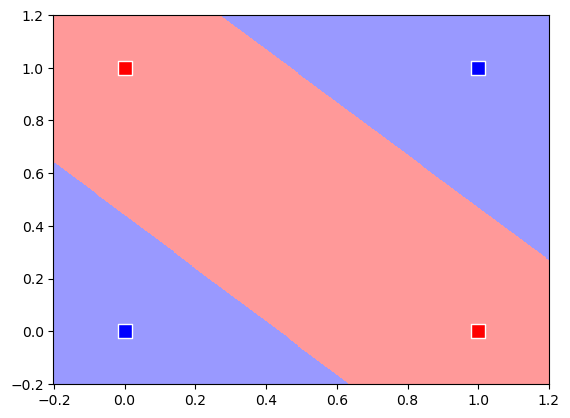
\includegraphics[height=0.6\linewidth]{Images/xor01}
				\label{fig:xor01}
			\end{figure}	
		\end{column}
	\end{columns}
	
\end{frame}

\begin{frame}{XOR Gate - Interpretation}
	\begin{columns}
		\begin{column}{0.4\textwidth}
			\begin{table}
				\centering
				\renewcommand{\arraystretch}{1.3} 
				\begin{tabular}{|c|c|c|c|c|}
					\hline
					\rowcolor{blue!80!black} 
					\textcolor{white}{\textbf{$x_1$}} & 
					\textcolor{white}{\textbf{$x_2$}} & 
					\textcolor{white}{\textbf{$h_1$}} & 
					\textcolor{white}{\textbf{$h_2$}} & 
					\textcolor{white}{\textbf{$\hat{y}$}} \\
					\hline
					0 & 0 & 1 & 1 & 0 \\
					\hline
					0 & 1 & 0 & 1 & 1 \\
					\hline
					1 & 0 & 0 & 1 & 1 \\
					\hline
					1 & 1 & 0 & 0 & 0 \\
					\hline
				\end{tabular}
			\end{table}
		\end{column}
		\begin{column}{0.6\textwidth}
			What exact Boolean operations are executed by:
			\begin{itemize}
				\item The first neuron of the hidden layer?
				\item The second neuron of the hidden layer?
				\item The single neuron at the output layer?
			\end{itemize}
		\end{column}
	\end{columns}
	
	\pause
	\vspace{0.3cm}
	
	\begin{itemize}
		\item The first hidden neuron implements a strict NOR gate:
		\begin{equation*}
			x_1, x_2 \mapsto \neg \left(x_1 \lor x_2\right)
		\end{equation*}
		\item The second hidden neuron implements a strict NAND gate:
		\begin{equation*}
			x_1, x_2 \mapsto \neg \left(x_1 \land x_2\right)
		\end{equation*}
		\item The output layer neuron performs an AND NOT operation on the hidden states: 
		\begin{equation*}
			h_1, h_2 \mapsto h_2 \land \left(\neg h_1 \right)
		\end{equation*}
	\end{itemize}
\end{frame}

\begin{frame}{XOR Gate - Mathematical Verification}
	Synthesizing the individual layers shows that the complete network implements:
	
	\begin{equation*}
		\begin{aligned}
			\hat{y} 
			&= h_2 \land \left(\neg h_1 \right) \\
			&= \left(\neg \left(x_1 \land x_2\right)\right) \land \neg \left( \neg \left(x_1 \lor x_2\right) \right) \\
			&= \left(\neg \left(x_1 \land x_2\right)\right) \land \left(x_1 \lor x_2\right) \\
			&= x_1 \oplus x_2
		\end{aligned}
	\end{equation*}
	
	The system successfully resolves the XOR function. Multiple alternative, valid weight spaces exist. For instance, the first neuron could have mapped to a standard OR gate instead of a NOR gate, requiring the output node to adapt and discover a standard AND gate.
	
	\vspace{0.3cm}
	
	Why doesn't the gradient optimization algorithm automatically pick the most \textit{intuitive} solution?
\end{frame}

\begin{frame}{XOR Gate - A Collaborative Effort!}
	While each hidden gate partitions its specific space linearly, the global combination overcomes linear boundaries:
	\begin{columns}
		\begin{column}{0.33\textwidth}
			\begin{figure}
				\centering
				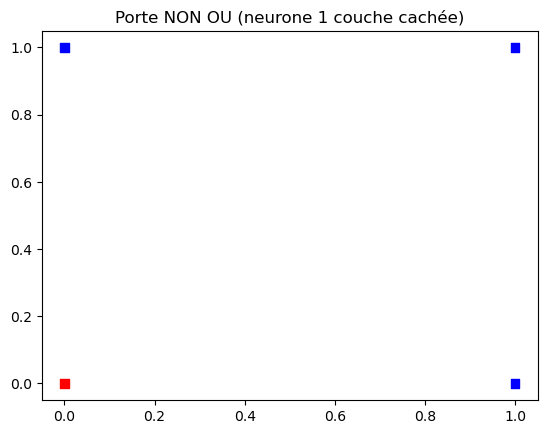
\includegraphics[height=0.85\linewidth]{Images/xor02}
				\label{fig:xor02}
			\end{figure}				
		\end{column}
		\begin{column}{0.33\textwidth}
			\begin{figure}
				\centering
				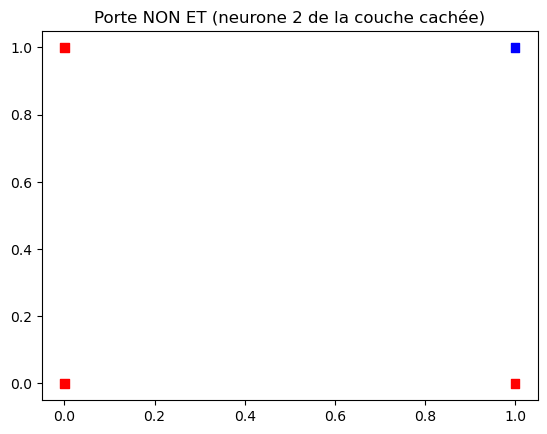
\includegraphics[height=0.85\linewidth]{Images/xor03}
				\label{fig:xor03}
			\end{figure}				
		\end{column}
		\begin{column}{0.33\textwidth}
			\begin{figure}
				\centering
				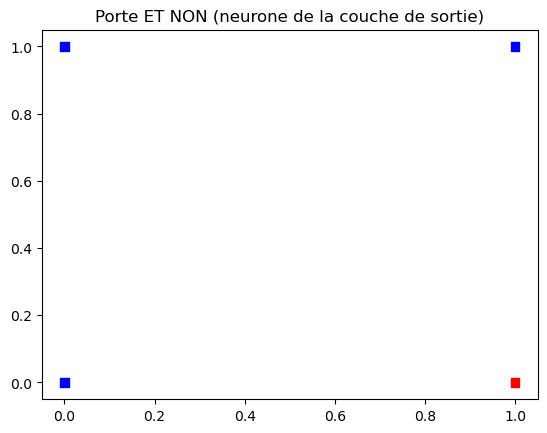
\includegraphics[height=0.85\linewidth]{Images/xor04}
				\label{fig:xor04}
			\end{figure}				
		\end{column}
	\end{columns}
	The hidden nodes act cooperatively like a team. Each unit solves an elementary linear task. By projecting these hidden features \textbf{non-linearly} through the \textbf{activation} function, the output layer untangles and correctly classifies the non-linear boundaries.
\end{frame}

\begin{frame}{XOR Gate - Latent Space Mapping}
	We can analyze this mechanism by examining the network's \textbf{latent space}. This space is defined by the axes $h_1$ and $h_2$ calculated across the training dataset:
	
	\begin{columns}
		\begin{column}{0.4\textwidth}
			\begin{figure}
				\centering
				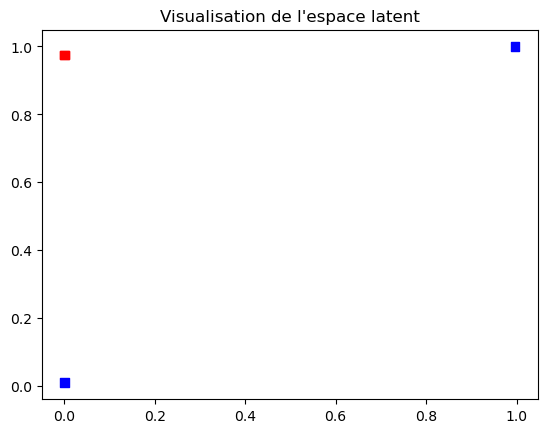
\includegraphics[height=0.9\linewidth]{Images/xor05}
				\label{fig:xor05}
			\end{figure}
		\end{column}	
		\begin{column}{0.6\textwidth}
			\begin{itemize}
				\item Within this latent coordinate system, the target labels become perfectly linearly separable. This geometric transformation is why the output node successfully completes the classification.
				\item The hidden layer has effectively \textit{warped} and stretched the coordinates of the initial input space. This non-linear transformation performs a powerful geometric \textbf{simplification} of the problem.
			\end{itemize}
		\end{column}
	\end{columns}
\end{frame}

\subsection[Activation Functions]{Activation Functions}

\begin{frame}{Choosing Activation Functions}
	It is standard practice to use different non-linear \textbf{activation functions} at separate layers within the network topology.
	\begin{itemize}
		\item The choice of activation function for the output layer is bound to the statistical nature of the target. For a \textbf{binary classification} task, the output $\hat{Y}$ must model a valid probability parameter; a \textbf{logistic} sigmoid function is the natural selection.
		\pause
		\item For multi-class classification tasks, employing a \textbf{softmax} operator at the output layer is required.
		\pause
		\item For a standard \textbf{regression} task, the output layer typically uses a linear identity activation. A single-layer network with a single linear node is therefore \textbf{strictly} identical to a classical \textbf{linear regression model}: $\hat{Y} = XW + b$.
		\pause
		\item For the hidden layers, three main activation functions have dominated the literature: the \textbf{logistic} function, the \textbf{hyperbolic tangent} ($\tanh$), and the Rectified Linear Unit (\textbf{ReLU}).
	\end{itemize}
\end{frame}

\begin{frame}{Conceptual Nature of Network Diagrams}
	\begin{alertblock}{Graphical Conventions for Activation Shapes}
		By convention, graphical diagrams of neural networks often draw a generic \textbf{sigmoid} curve within the nodes as a general placeholder for non-linearity. One must always consult the exact mathematical configuration of each layer; these visual symbols are purely \textbf{conceptual}.
	\end{alertblock}
\end{frame}

\begin{frame}{The Logistic Function}
	\begin{block}{Logistic Sigmoid Function}
		The \textbf{logistic} function is a smooth mapping $\sigma: \R \to (0, 1)$ defined as:
		
		\begin{equation*}
			\sigma: z \mapsto \frac{1}{1 + e^{-z}}
		\end{equation*}
		
		It serves as a smooth, continuously differentiable alternative to the Heaviside step function. While widely deployed at the output layer for \textbf{binary classification}, it can also be configured within hidden layers.
	\end{block}
	
	\begin{figure}
		\centering
		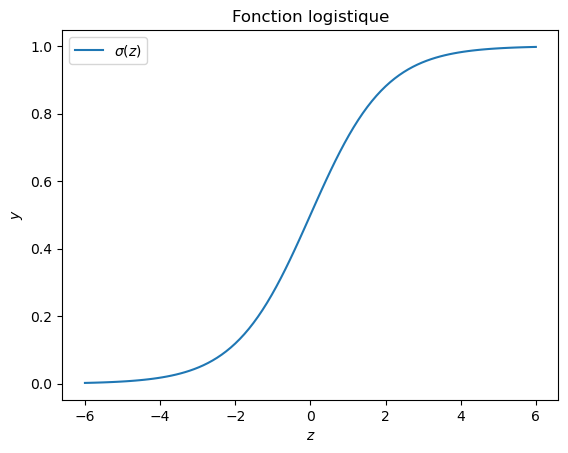
\includegraphics[height=0.25\linewidth]{Images/nonlinearites02}
		\label{fig:nonlinearites02}
	\end{figure}	
\end{frame}

\begin{frame}{The Softmax Function}
	\begin{block}{Softmax Transformation}
		The \textbf{softmax} function maps a multivariate vector input $\operatorname{softmax}: \R^p \to (0, 1)^p$ according to the following expression:
		
		\begin{equation*}
			\operatorname{softmax}: z_j \mapsto \frac{e^{z_j}}{\sum_{i=1}^{p} e^{z_i}} \; \forall \; j = 1, 2, \cdots, p
		\end{equation*}
		
		It generalizes the logistic function to \textbf{multi-class classification} problems and is restricted to the final layer. It mathematically guarantees the following probability normalisation constraint:
		
		\begin{equation*}
			\sum_{j=1}^p \operatorname{softmax}\left(z_j\right) = 1
		\end{equation*}
	\end{block}
\end{frame}

\begin{frame}{Softmax and Numerical Stability}
	\begin{block}{Numerically Stable Softmax Implementation}
		The raw theoretical formulation of the \textbf{softmax} function is unstable on computer hardware due to floating-point overflow. Production libraries implement the following stable mathematical equivalent instead:
		
		\begin{equation*}
			\operatorname{softmax}: z_j \mapsto \frac{e^{z_j - z_{\text{max}}}}{\sum_{i=1}^{p} e^{z_i - z_{\text{max}}}} \; \forall \; j = 1, 2, \cdots, p
		\end{equation*}
		
		Where $z_{\text{max}}$ denotes the maximum element within the input vector $z$:
		
		\begin{equation*}
			z_{\text{max}} = \underset{i}{\max{\left(z_i\right)}} \; \text{;} \; i = 1, 2, \dots, p
		\end{equation*}
		
		This translation trick bounds the exponential calculations, preventing capacity overflow errors.
	\end{block}
\end{frame}


\begin{frame}{The Hyperbolic Tangent Function}
	\begin{block}{Hyperbolic Tangent ($\tanh$)}
		The \textbf{hyperbolic tangent} is a smooth mapping $\tanh: \R \to (-1, 1)$ defined as:
		
		\begin{equation*}
			\tanh: z \mapsto \frac{1 - e^{-2 z}}{1 + e^{- 2 z}}
		\end{equation*}
		
		Functional behaviors mirror the logistic function, but the range is zero-centered between $-1$ and $1$. It represents the \textbf{historical} default activation function for traditional \textbf{dense} network layers.
		
	\end{block}
	
	\begin{figure}
		\centering
		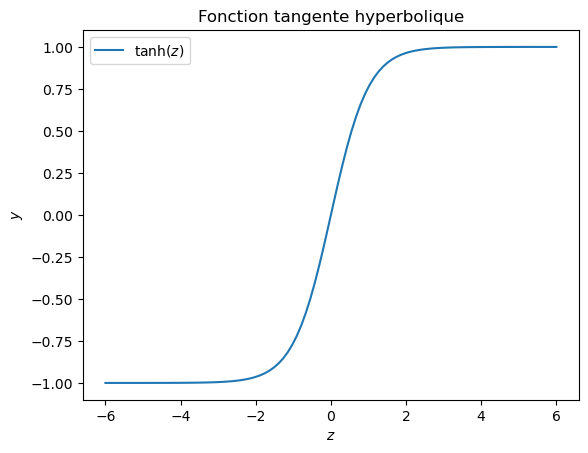
\includegraphics[height=0.25\linewidth]{Images/nonlinearites03}
		\label{fig:nonlinearites03}
	\end{figure}		
\end{frame}

\begin{frame}{The Rectified Linear Unit (ReLU)}
	\begin{block}{Rectified Linear Unit Function: ReLU}
		The \textbf{Rectified Linear Unit} or \textbf{ReLU} function is a piecewise linear mapping $\operatorname{ReLU}: \R \to [0, +\infty[$ defined as:
		
		\begin{equation*}
			\operatorname{ReLU}: z \mapsto \begin{cases}
				z & \text{if } \; z > 0 \\
				0 & \text{otherwise}
			\end{cases}
		\end{equation*}
		
		Despite a point of non-differentiability located precisely at zero, it has become the universal default standard for training modern deep neural architectures.
		
	\end{block}
	\vspace{-0.2cm}
	
	\begin{figure}
		\centering
		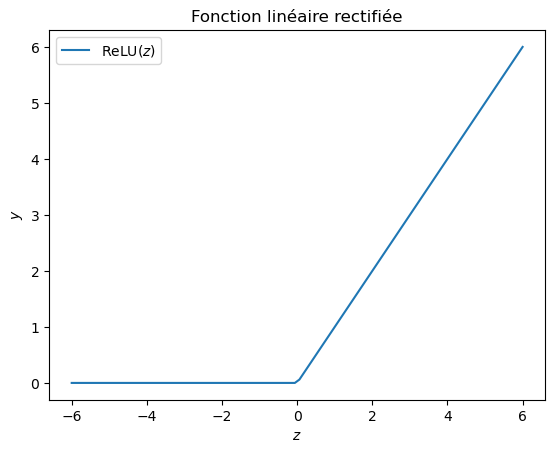
\includegraphics[height=0.28\linewidth]{Images/nonlinearites04}
		\label{fig:nonlinearites04}
	\end{figure}		
\end{frame}

\begin{frame}{Choosing Hidden Layer Activation Functions}
	For hidden layers:
	\begin{itemize}
		\item Selecting the specific activation function behaves as a structural architectural \textbf{hyperparameter}.
		\pause
		\item The final choice is typically determined empirically via rigorous \textbf{cross-validation} loops.
		\pause
		\item The ReLU function exhibits superior empirical performance on deep models with high layer counts, as it effectively mitigates the vanishing gradient problem.
		\pause
		\item Logistic curves and hyperbolic tangents retain high effectiveness on simpler, shallower network configurations. The logistic function is now mostly restricted to output layer probabilities.
	\end{itemize}
\end{frame}

\begin{frame}{Feature Engineering vs. Network Architecture}
	With linear and logistic regression models, we saw that solving non-linear boundaries required designing an explicit expansion mapping $\Phi: \mathcal{X} \to \tilde{\mathcal{X}}$ to manually inject non-linear combinations of the inputs $X$.
	
	\vspace{0.5cm}
	\pause
	
	In the connectionist approach, non-linear representation capacity is completely delegated to structural hyperparameters:
	\begin{itemize}
		\item The choice of activation functions (the mathematical engine of non-linearity).
		\item The total depth of the layers.
		\item The node density per hidden layer.
	\end{itemize}
	
	\vspace{0.5cm}
	\pause
	
	Which philosophy is more robust? Which approach should we prioritize?
\end{frame}

\begin{frame}{Feature Engineering vs. Network Architecture}
	In real-world data science engineering, the optimal path combines \textit{both}:
	
	\begin{itemize}
		\item Designing the expansion function $\Phi$ leverages critical domain-specific \textbf{expertise}. This workflow is called \textbf{feature engineering}. If physical theory states that a target variable scales with the square of an input feature, it is always more efficient to inject that squared term explicitly rather than forcing the network layers to poorly \textbf{reconstruct} that specific quadratic behavior from raw numerical data.
		\pause
		\item Conversely, hidden feature interactions are often too intricate for an expert to manually design. Neural networks excel at automatically \textbf{discovering} and isolating these latent structural patterns for us.
		\pause
		\item The principle of parsimony (\textbf{simplicity}) must remain our guide. Smart, elegant \textbf{feature engineering} shrinks required network complexity. For small sample sizes, this parameter reduction lowers global model \textbf{variance}. By infusing domain knowledge, feature engineering also protects the model against structural \textbf{bias}.
	\end{itemize}	
\end{frame}

\begin{frame}{The Forward Pass Layer Transformation}
	
	\begin{block}{Forward Pass in a Dense Layer}
		To mathematically summarize a single \textbf{forward pass} through a dense layer during inference or \textbf{prediction}:
		
		\begin{equation*}
			X \mapsto \sigma\left(X W + b\right)
		\end{equation*} 
		
		It is fundamentally the composition of an affine transformation (\textbf{linear}) followed by a coordinate mapping projection (\textbf{non-linear}).		
	\end{block}
	
	\vspace{0.3cm}
	
	Note: For the remainder of this course, the generic symbol $\sigma$ will denote any chosen activation function (logistic, hyperbolic tangent, or ReLU).
	
\end{frame}